\fig{fv:k1:time}{一小段位移的用时对应倒速度图下的窄条面积}{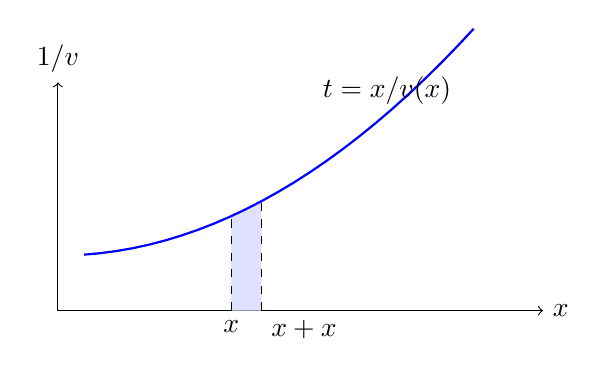
\begin{tikzpicture}[x=1.1cm,y=1cm]
\draw[->](0,0)--(5.6,0)node[right]{$x$};\draw[->](0,0)--(0,2.9)node[above]{$1/v$};
\fill[blue!12](2,0)--(2,1.2)--(2.35,1.39)--(2.35,0)--cycle;
\draw[blue,thick,domain=.3:4.8]plot(\x,{.7+.125*\x*\x});
\draw[dashed](2,0)--(2,1.2);\draw[dashed](2.35,0)--(2.35,1.39);
\node[below]at(2,0){$x$};\node[below right]at(2.35,0){$x+\dd x$};
\node at(3.8,2.8){$\dd t=\dd x/v(x)$};\end{tikzpicture}}
图\ref{fv:k1:time}中的横向小段仍是实际位移，纵向高度却是倒速度。因此低速区域在图上更高，对总用时的贡献更大。若 $v(x)$在某点趋零，不能只看路程有限就认定用时有限，应检查倒速度积分是否收敛。图示只覆盖 $v>0$的单调运动段；发生反向后，应另分一段并按实际方向计算时间。
